%% We use `subfiles' package
\documentclass[preamble.tex]{subfiles}
\begin{document}

\clearpage

\chapter{Introduction}
\label{ch:introduction}

The past decade has seen a rise in development of increasingly sophisticated multi-core and multi-processor computer systems. From the early hyperthreaded solutions to the modern architectures comprising of a number of independent processing cores, the horsepower for demanding applications is now available even in the most affordable consumer systems. To offer a large amount of parallelism the high grade systems may have multiple multi-core processors, where each of the cores can run a number of hardware scheduled threads.

While the hardware for running highly parallel computations is available and is improving at a high pace, the development of such applications targeting an arbitrary number of processing elements\ipe{}\footnote{A processing element is taken to be a processor, a processor's core, a hardware thread or a combination of the above.} is often a challenging task. The problems involved are finding an appropriate parallel implementation of the task at hand, implementing it such that the computations are evenly distributed across processing elements and synchronising parallel computations when necessary. The latter two require a substantial programmer's intervention to get the algorithm running fast.

% It is not uncommon for the initial parallel implementation to run only slightly faster than the sequential version.

The resulting application is a mixture of the actual algorithm and the implementation specific code, dealing with concurrency and parallelism. This obscures code clarity and may generally be error-prone.

One alternative to this practice of explicit parallelisation is to provide a common set of collective operations\icollop{} on large data structures. Programs implemented in terms of these operations would be automatically parallelised across the available processing elements. This approach is successfully exercised by a multitude of frameworks covering many host languages, target architectures and suitable applications domains \cite{PLKC08,KCL+10,CKL+11,AS07}.

However, in the pursuit of a high level approach to programming a major inefficiency is introduced. Having provided a number of collective operations, the problem of multiple traversals arises. In each program there is likely to be a number of such operations composed together in some way to compute the desired result. With each collective operation potentially traversing a large data structure, the memory traffic is considerably increased.

In a program written by hand without the use of collective operations the programmer would naturally recognise all the operation that could be performed in one pass over the data structure. The program would only traverse the data structure as few times as required, keeping the memory traffic to the necessary minimum and utilising cache correctly.

On the other hand using a straight-forward implementation of a high level library of collective operations would result in code that traverses data which performing only a small change in each pass. For large data structures this may lead to poor cache utilisation and high memory traffic, noticeably reducing the overall performance.

Additionally, each operation may need to store its result in a new data structure, which is especially true for languages where values are immutable by default. Allocating temporary data structures to store the intermediate results\index{intermediate value}{} leads to further memory and runtime penalties.

Optimising out the superfluous data structure traversals and allocations is collectively referred to as \name{Loop Fusion}\ifusion{}. It allows to transform a program expressed in terms of high level operations into a program that would be comparable to a handwritten one in operation and speed.

In this essay I explore the problem of \name{loop fusion} in the context of purely functional data parallel programs. I shall begin by introducing the reader to the context of my work. I outline the problem finding a solution to which, has motivated my work in the prior years.

\clearpage


\section{What is Array Fusion?}

Suppose we have the following computation to perform:

\begin{hscode}
sum (zipWith (*) xs ys)
\end{hscode}

A person familiar with the fundamentals of functional programming is likely to spot the computation of the dot product of two vectors in this snippet of \Haskell code. Indeed, the @zipWith@ list combinator\icomb{} will element-wise multiply the two vectors @xs@ and @ys@. Quite expectedly the @sum@ combinator will sum the elements of the resulting vector into a scalar value yielding the dot product of @xs@ and @ys@.

This one-liner was an attempt to develop the motivation for the high-level view on numeric computations. It may seem reasonable to replace the lists with arrays and reimplement the same high-level interface in terms of traditional arrays to avoid random memory access penalties as in the case of lists.

Providing an instantly familiar interface without compromising performance has been one of the goals of the \name{Data Parallel Haskell (DPH)}\idph{} project \cite{PLKC08,CLP+07}. The work described in this essay has been carried out in the context of this project. It will be discussed in more detail in section \ref{sec:DPH}.

However, even if we replaced the lists with arrays and gave efficient implementations to @sum@ and @zipWith@, the resulting algorithm is still likely to be slower than one written by hand in a language such as \C. The @zipWith@ combinator \*produces* an \*intermediate array*\iintermediate{} containing the element-wise product of the two input vectors. It is immediately \*consumed* by @sum@, yielding the final (scalar) value. Thus the algorithm performs two traversals and allocates another array of the size of the input arrays.

To illustrate the benefit of Array Fusion let us turn to the implementation of same algorithm expressed in \C:


\begin{ccode}
double dotProduct (double xs[], double ys[], int len) {
	// zipWith
	double* temp = malloc(len * sizeof(double));
	for(int i = 0; i < len; i++)
		temp[i] = xs[i] * ys[i];

	// sum
	double result = 0;
	for(int i = 0; i < len; i++)
		result += temp[i];

	return result;
}
\end{ccode}


We immediately notice that both loops iterate over the same \*range* of indices and we could hence perform it as one loop. The two loops are said to have the same \*rate*\irate{} (the term used more recently in the context of loop fusion in \Haskell \cite{BenLippmeier:2014jc}).


\begin{ccode}
double* temp = malloc(len * sizeof(double));
double result = 0;
for(i = 0; i < len; i++) {
	temp[i] = xs[i] * ys[i];
	result += temp[i];
}
\end{ccode}


\begin{bluebox}
The process of finding and exploiting the opportunities for merging multiple loops into one is referred to as \term{loop fusion}\ifusion{}.
\end{bluebox}


However, this does not completely bypass the allocation of an intermediate array\iintermediate{}. Clearly, the intermediate array is redundant and the intermediate value @temp@ could just be a \*scalar* as in the following:


\begin{ccode}
double temp; // temp has become scalar
double result = 0;
for(int i = 0; i < len; i++) {
	temp = xs[i] * ys[i];
	result += temp;
}
\end{ccode}


\begin{bluebox}
The optimisation that removes the need for temporary arrays by replacing them with scalars is called \term{scalarisation}\index{scalarisation}{}.
\end{bluebox}


It is a special case of \term{array contraction}\index{array contraction}{}. Array contraction optimisation attempts to remove a \*dimension* from the array. In this particular case we contracted a one dimensional array to a scalar, hence \*scalarisation*. However, in the examples with arrays of higher dimensions the dimension could just be reduced, and not eliminated entirely. We will see examples of that in the upcoming chapters when we discuss \*segmented array combinators*\isegmented. This concept is taken even further in multi-dimensional array systems such as \name{Repa} \cite{KCL+10} and \name{Accelerate} \cite{CKL+11}.


\begin{bluebox}
\term{Loop Fusion} and \term{Array Contraction} optimisation are collectively referred to as \term{Array Fusion}.
\end{bluebox}


Another term for this commonly encountered in literature is \term{deforestation}\index{deforestation}{}, first coined by Philip Wadler in \cite{Wad90}.

The work described in this thesis is aimed at introducing a new fusion mechanism in \name{Data Parallel Haskell (DPH)}\idph{} framework. In following section I will introduce the reader to the \DPH project. I will then describe some of the most common fusion systems and identify their shortcomings which motivated the search for a fresh approach.



\clearpage

\section{Data Parallel Haskell}
\label{sec:DPH}

\name{Data Parallel Haskell (DPH)}\idph{} is a library for and an extension to the \Haskell programming language, providing high level access to \*nested data parallelism*. The above definition may seem complicated at first and should probably be backed up by a set of explanations:

\term{Nested data parallelism}\index{data parallelism: nested}{} is a type of \name{SPMD}\index{data parallelism: SPMD (single program, multiple data)}{} parallelism (single program, multiple data) which operates on \*irregular*\index{data structure: irregular} data structures. Two examples of irregular data structures are \*sparse matrices*\index{data structure: sparse matrix} and \*unbalanced trees*\index{data structure: unbalanced tree}.

In a nested data parallel program parallel computations can call further data parallel computations. For example when traversing an unbalanced tree each node may process each of its children in parallel. Without statically knowing the branching of the tree, it may be difficult to adequately parallelise the process. \DPH offers an elegant solution through its vectorisation process which will be discussed in Section \ref{sec:Vectorisation}.

\DPH takes an active part in the optimisation and the compilation of its client code. It guides the compilation process in many ways including vectorisation \cite{PLKC08}, choosing the optimal data representation \cite{CDL09} as well as applying fusion \cite{CLP+07} and rewrite rules \cite{PTH01} to improve performance.

In essence \DPH reimplements the familiar list interface in terms of seamlessly parallelised arrays. Listing \ref{fig:DPH-interface} shows some of the most important functions in the \DPH interface. Since \DPH has language support, the bracket notation for parallel arrays closely resembles that for \Haskell lists: @[:a:]@ denotes a parallel array of type @a@, while @[:[:a:]:]@ is a nested parallel array. The counterpart of \Haskell's list comprehensions is also present and is called \*parallel array comprehensions*.


\begin{hscode2}{Type signatures for parallel array operations. \label{fig:DPH-interface}}
(!:)         :: [:a:] -> Int -> a
sliceP       :: [:a:] -> (Int,Int) -> [:a:]
replicateP   :: Int -> a -> [:a:]
mapP         :: (a -> b) -> [:a:] -> [:b:]
zipP         :: [:a:] -> [:b:] -> [:(a,b):]
zipWithP     :: (a -> b -> c) -> [:a:] -> [:b:] -> [:c:]
filterP      :: (a -> Bool) -> [:a:] -> [:a:]

concatP      :: [:[:a:]:] -> [:a:]
concatMapP   :: (a -> [:b:]) -> [:a:] -> [:b:]
unconcatMapP :: [:[:a:]:] -> [:b:] -> [:[:b:]:]
transposeP   :: [:[:a:]:] -> [:[:a:]:]
expandP      :: [:[:a:]:] -> [:b:] -> [:b:]

combineP     :: [:Bool:] -> [:a:] -> [:a:] -> [:a:]
splitP       :: [:Bool:] -> [:a:] -> ([:a:], [:a:])
\end{hscode2}


Collective operations on parallel arrays are executed in parallel when the hardware supports it. The framework is targeting shared memory architectures and currently uses \Haskell threads \cite{Jones08atutorial} to achieve parallelism.

By design the computation is split evenly across processing elements even for highly irregular parallel programs. The next section will outline the library structure, cover the basics of vectorisation and describe the current stages of fusion in \DPH.



\subsection{Vectorisation}
\label{sec:Vectorisation}
\ivect{}

The principle idea behind \DPH was to allow the programmer write parallel programs without the additional effort of parallelising, scheduling, load balancing and low level optimisation.

The work on \DPH was originally inspired by Blelloch's pioneering work on \name{NESL} \cite{BCH+}, a research language designed to explore the new approach to nested data parallelism.

At the core of \DPH is the vectoriser which is implemented in the \name{Glasgow Haskell Compiler}\footnote{Glasgow Haskell Compiler: http://www.haskell.org/ghc} (\GHC).

\begin{bluebox}
\name{Vectoriser} transforms \term{nested} data parallelism to \term{flat} data parallelism by means of \term{flattening transform} on \*data* and \term{lifting transform} on \*functions*.
\end{bluebox}

The two transforms are described below:


\subsubsection{Flattening transform (on data)}

\begin{figure}
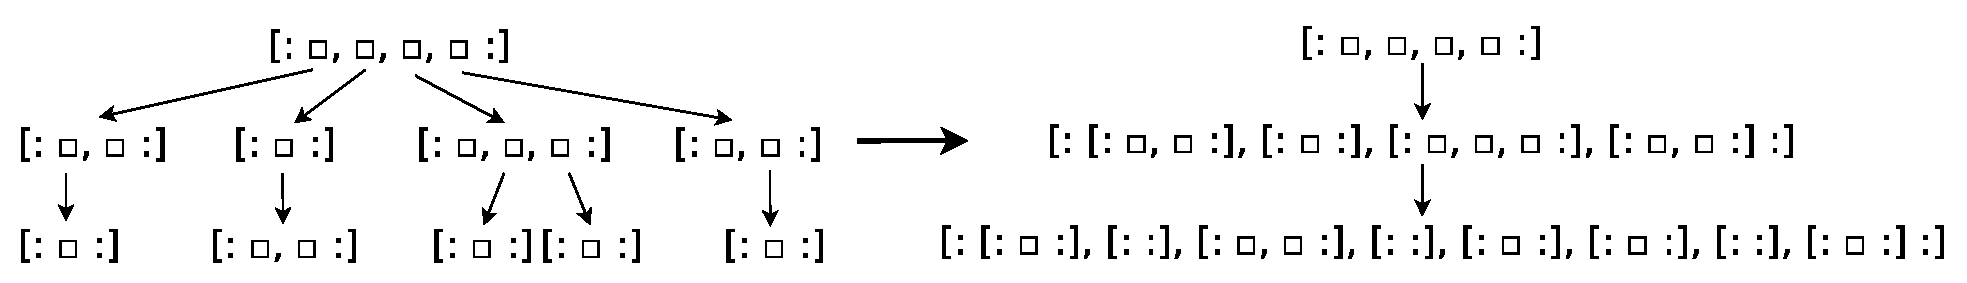
\includegraphics[width=1\textwidth]{img/TreeRepr}
\caption{Value of type \code{[:Tree:]} and its vectorised representation. Empty subtrees are omitted from the conceptual representation.%
\label{fig:Tree}}
\end{figure}


If we were to take a tree\index{data structure: tree}{} of an arbitrary shape and tried to apply some computation to its every node in parallel, a naive tree representation would have probably failed to provide us with enough clues on how to split the load between processing elements. Suppose we store an element of type \texttt{Int} and an array of subtrees at each node. Then the tree can be expressed as

\begin{hscode}
data Tree = Tree Int [:Tree:]
\end{hscode}


A sample tree is given in Figure \ref{fig:Tree}. Just by looking at the top level of the tree it would not be possible to know the branching. What vectorisation does is it translates user programs that use nested data parallelism to those using flat data parallelism. Figure \ref{fig:Tree} presents the same tree with each of its levels placed into a parallel array. At the implementation level it is flattened even further by storing a flat data array with all the node values and a \*segment descriptor*\isegd{} defining the partitioning to recreate the original nesting. Thus, a parallel array with elements $[: [:5:],[::],[:4,2:],[::],[:3:],[:17:],[::],[:11:] :]$

\begin{lstlisting}[basicstyle={\ttfamily},language=Haskell]
[: [:5:],[::],[:4,2:],[::],[:3:],[:17:],[::],[:11:] :]
\end{lstlisting}


which may have been the deepest level of the discussed tree, would have been stored as an array of unboxed values

\begin{lstlisting}[basicstyle={\ttfamily},language=Haskell]
[# 5, 4, 2, 3, 17, 11 #]        -- data
\end{lstlisting}


together with the segment descriptor containing the lengths and the starting index positions of the contained arrays (offsets into the data array):

\begin{lstlisting}[basicstyle={\ttfamily},language=Haskell]
([# 1, 0, 2, 0, 1, 1, 0, 1 #],  -- lengths
 [# 0, 1, 1, 3, 3, 4, 5, 5 #])  -- indices
\end{lstlisting}



\subsubsection{Data Representation}
\label{sub:DPH-Data-Representation}

Together with flattening, the vectoriser chooses the best representation for the data, e.g. for sum types and product types. \Haskell's product types, or the tuples of two of more heterogeneous elements, are allocated as boxed values on the heap. Storing an array of pointers to heap allocated values would have been a major hit on performance due to the costs of unboxing as well as loading the individual values from memory instead of fetching multiple at a time. Instead, an array of pairs \texttt{{[}:(a,b):{]}} is stored as a pair of arrays \texttt{({[}:a:{]},{[}:b:{]})}.

Similarly, the sum types, or the user defined ADT's, are stored as tuples of arrays. Having multiple arrays, each storing the interesting values wrapped by the same constructor, not only avoids the cost of unboxing but also facilitates pattern matching on constructors. Thus the values constructed by the same constructor are stored in the same array. The penalty paid is keeping a selector array to recreate the original interleaving. Quite clearly sum types and product types can be recursively nested.%


\begin{comment}
TODO: give an example of sum types and their representation in parrs
\end{comment}

\subsubsection{Lifting transform (on functions)}
We have discussed the way the data is represented in DPH but said nothing about how the vectoriser adapts the functions to fit the new data representation. We do not need to delve into too much detail here, since by the time we get to the backend of the library (where the fusion takes place) we are no longer interested in how it's done. One important intuition to develop can be illustrated by the following:

\begin{hscode}
f :: Float -> Float
f x = x*x + 1
\end{hscode}


For every such function the vectoriser generates its \emph{lifted }version \texttt{f\textasciicircum{}} thus:

\begin{lstlisting}[basicstyle={\ttfamily},language=Haskell]
f^ :: [:Float:] -> [:Float:] -> [:Float:]
f^ x = (x *^ x) +^ (replicateP n 1)
       where n = lengthP x
\end{lstlisting}


This new definition obeys the equation \texttt{f\textasciicircum{} = mapP f}, thus it is possible to replace \texttt{(mapP f)} with \texttt{f\textasciicircum{}}. Now if we return to the tree example, there we may need to apply \texttt{f }to an array of arrays. The flat data representation we chose above allows us to easily derive \texttt{f\textasciicircum{}\textasciicircum{}} in terms of \texttt{f\textasciicircum{}} like this:

\begin{lstlisting}[basicstyle={\ttfamily},language=Haskell]
f^^ :: [:[:Float:]:] -> [:[:Float:]:]
f^^ xss = unconcatP xss (f^ (concatP xss))
\end{lstlisting}


Recalling that we use a flat data array together with a segment descriptor to represent \texttt{xss}, it becomes clear that both \texttt{concatP} and \texttt{unconcatP} are simple constant time operations that do nothing more than replacing one segment descriptor with another.

Vectorisation is more thoroughly covered in the tutorial-style paper \cite{PLKC08}.


\section{Backend and Fusion}

By the time the backend is reached the nesting in the original user program is only defined in terms of segment descriptors where required. As discussed in the previous section the vectoriser has also stripped out the product and sum types including those defined by the user and conveniently arranged them in flat data arrays. Thus, the backend, or the library of primitive operations, needs only support the arrays of primitive types. Since some of the operations on nested arrays need to respect the boundaries of the inner arrays (e.g. reductions), the segmentation information is still present.

The primitive library implements a fixed interface that is called by the vectoriser. The support for any architectures other than multi-core systems can be added through reimplementing the primitive library interface, though the parallel programming model heavily relies on shared memory architectures for efficiency. The primitive library in its current state uses the Vector library\footnote{http://hackage.haskell.org/package/vector } to store arrays and Haskell threads to implement parallelism \cite{Jones08atutorial}. Essentially each thread is given a chunk of array(s) and a sequential operation to apply to it.

\label{Lit:DPH-fusion-levels}DPH introduces fusion at three different
levels:
\begin{enumerate}
\item Removing synchronisation points\\ Due to the use of Haskell threads, the code responsible for distributing the processing across the processing elements introduces many fork/join points. Due to the specifics of the other two fusion levels, this does not allow the fusion to be applied. Thus, if there is no processing to be done between the join and the next fork, these are fused together using the rewrite rules \cite{PTH01}. One problem with this approach is that the rewrite happens unconditionally when matched, which may lead to unbalanced load, e.g. after a \texttt{filter} operation.
\item A minimal set of sequential rewrite rules\\ Just like removing superfluous synchronisation points, some adjacent array operations can be optimised away with the help of rewrite rules. An example of an easy optimisation would be on two consecutive maps on the same array, i.e. \texttt{map f (map g xs) = map (f . g) xs}. While these optimisations are quick and effective, it is not feasible to come up with a rewrite rule for every pair of fusible operations. A small set of such rewrite rule is employed in DPH to get rid of the most common combinations at a relatively low cost.
\item Stream Fusion\\ Stream fusion receives the most attention as far as the fusion in DPH goes. It not only considerably affects the internal implementation of primitive operations in DPH and in the Vector library, but also relies on a certain set of optimisations in the compiler. It will be described in a later section. Like the two previous fusion rules, this one also includes a rewrite rule which triggers the optimisation.
\end{enumerate}


Unfortunately, the common point of failure of all of the above fusion types is that they rely on the consecutive operations being inlined and always following each other with nothing in between. This is a necessary condition for the rewrite rules to fire.


\IfNotCompilingAll{\bibliography{bib}}


\end{document}